% ju 26-Dez-22
\documentclass[a4paper,12pt,fleqn,parskip=half]{scrartcl}
\usepackage[ngerman]{babel}
\usepackage[utf8]{inputenc}
\usepackage[T1]{fontenc}

% Schrift
%\usepackage{lmodern}
\usepackage[osf,sc]{mathpazo} 
\usepackage[scale=.9,semibold]{sourcecodepro}   
\usepackage[osf]{sourcesanspro}  

\usepackage[headsepline]{scrlayer-scrpage}
\pagestyle{scrheadings}
\clearpairofpagestyles

\usepackage[table,dvipsnames,usenames]{xcolor}
\usepackage{textcase}
\usepackage{nameref}
\usepackage{hyperref}
\usepackage{tabularx}
\usepackage{multirow}
\usepackage{multicol}
\usepackage{caption, booktabs}
\usepackage{graphicx} 
\usepackage{scrhack}    
\usepackage{url}%% Links
\usepackage[inline]{enumitem}
\usepackage{pifont}
\usepackage{eurosym}% \euro 20,-
\usepackage{amsmath}
\usepackage{amsfonts}
\usepackage{amssymb}
\usepackage{array}            % Extending the array and tabular environments
\usepackage{chngcntr}         % Change the resetting of counters
\usepackage[version=4]{mhchem}
\usepackage{stmaryrd}
\usepackage{siunitx}
\usepackage{float}
\usepackage{csquotes}
\usepackage{subcaption}
\usepackage{mathtools}
\usepackage{icomma}%Dezimaltrennzeichen
\usepackage{multimedia}%Video: \movie[externalviewer]{(video.mov)}{video.mov}
\usepackage{epstopdf}
\usepackage{footnote}
\usepackage{qrcode}% Anwendung: \qrcode[hyperlink,level=Q,version=2,height=1cm]{\website}
\usepackage{underscore}% Unterstrich ____

% PDF Dokumente einbinden
\usepackage{pdfpages}% \includepdf[pages=-]{Tabellen/Excel.pdf}
\RequirePackage{lastpage}  % Pagecounter

\addto\captionsngerman{%
\renewcommand{\figurename}{Abb.}
\renewcommand{\tablename}{Tab.}
}

% listings
\usepackage{listings}
\lstset{basicstyle=\linespread{1}\ttfamily\small,floatplacement=!htb,captionpos=t,abovecaptionskip=.5\baselineskip,belowcaptionskip=.5\baselineskip,upquote=true,showstringspaces=false,inputencoding=utf8,tabsize=4,
    	keywordstyle=\bfseries ,
	commentstyle=\color{rot5},
	stringstyle=\color{orange},
	breaklines=true,
  	postbreak=\mbox{\textcolor{black}{$\hookrightarrow$}\space},
	breakatwhitespace=false
}
\lstset{literate={á}{{\'a}}1 {é}{{\'e}}1 {í}{{\'i}}1 {ó}{{\'o}}1 {ú}{{\'u}}1 {Á}{{\'A}}1 {É}{{\'E}}1 {Í}{{\'I}}1 {Ó}{{\'O}}1 {Ú}{{\'U}}1 {à}{{\`a}}1 {è}{{\`e}}1 {ì}{{\`i}}1 {ò}{{\`o}}1 {ù}{{\`u}}1 {À}{{\`A}}1 {È}{{\'E}}1 {Ì}{{\`I}}1 {Ò}{{\`O}}1 {Ù}{{\`U}}1 {ä}{{\"a}}1 {ë}{{\"e}}1 {ï}{{\"i}}1 {ö}{{\"o}}1 {ü}{{\"u}}1 {Ä}{{\"A}}1 {Ë}{{\"E}}1 {Ï}{{\"I}}1 {Ö}{{\"O}}1 {Ü}{{\"U}}1 {â}{{\^a}}1 {ê}{{\^e}}1 {î}{{\^i}}1 {ô}{{\^o}}1 {û}{{\^u}}1 {Â}{{\^A}}1 {Ê}{{\^E}}1 {Î}{{\^I}}1 {Ô}{{\^O}}1 {Û}{{\^U}}1 {œ}{{\oe}}1 {Œ}{{\OE}}1 {æ}{{\ae}}1 {Æ}{{\AE}}1 {ß}{{\ss}}1 {ű}{{\H{u}}}1 {Ű}{{\H{U}}}1 {ő}{{\H{o}}}1 {Ő}{{\H{O}}}1 {ç}{{\c c}}1 {Ç}{{\c C}}1 {ø}{{\o}}1 {å}{{\r a}}1 {Å}{{\r A}}1 {€}{{\EUR}}1 {£}{{\pounds}}1 {~}{{\textasciitilde}}1 {-}{{-}}1 }

% bibliography
\usepackage[
    bibencoding=utf8,
    backend=biber,% bibtex, biber
    backref=false,backrefstyle=three+,url=true,urldate=comp,abbreviate=false,maxnames=20
]{biblatex} %Paket laden
\DeclareBibliographyCategory{cited}
\let\defaultcite\cite\renewcommand*\cite[2][]{\addtocategory{cited}{#2}\defaultcite[#1]{#2}}
\let\defaulttextcite\textcite\renewcommand*\textcite[2][]{\addtocategory{cited}{#2}\defaulttextcite[#1]{#2}}
\setcounter{biburllcpenalty}{7000}
\setcounter{biburlucpenalty}{8000}
\AfterPackage{biblatex}{
	\PreventPackageFromLoading[\errmessage{Sie haben versucht, das Cite-Paket zu laden, das nicht mit biblatex kompatibel ist.}]{cite}
}

\hypersetup{%
	%pdftitle={\titel},
	%pdfsubject={Latex},
	%pdfauthor={\autor},
	%pdfcreator={\autor}, 
	bookmarksnumbered=true,
	breaklinks=true,
	%colorlinks=true,	   
	linkcolor=rot5,		
	filecolor=blau5,		
	urlcolor=blau5,			
	citecolor=ForestGreen
}

\linespread{1.1}
\setlist{itemsep=0pt}
\widowpenalty10000
\clubpenalty10000
\tolerance1000   

\usepackage[left=2cm,right=2cm,top=1cm,bottom=1cm,includeheadfoot]{geometry}
%\usepackage[left=4cm,right=2cm,top=1cm, bottom=1cm,includeheadfoot]{geometry}
%\usepackage[left=6cm,right=1cm,top=1cm, bottom=1cm,includeheadfoot]{geometry}
%\usepackage[landscape=true,left=2cm,right=2cm,top=1cm,bottom=1cm,includeheadfoot]{geometry}%quer

% eigene Farbe definieren
% Adobe Prozessfarben: CMYK: 100,50,0,35 -> 1,0.5,0,0.35
\definecolor{orange}{cmyk}{0,0.55,0.61,0}   % 0,55,61,0
\definecolor{blau5}{cmyk}{1,0.77,0.1,0.01}  % 100,77,10,
\definecolor{rot5}{cmyk}{0.22,1,1,0.19}     % 22,100,100,19
\definecolor{grau2}{cmyk}{0,0,0,0.1}        % 0,0,0,40
\definecolor{blau}{cmyk}{0.93,0.66,0,0.21}% 

% Literatur
\bibliography{content/literatur}
\bibliography{content/literatur-kfz}
\bibliography{content/literatur-sport}

%%%%%%%%%%%%%%%%%%%%%%%%%%%%%%%%%%%%%%%%%%%%%%%%%%%%%%%
\newcommand{\name}{Jan Unger}
\newcommand{\thema}{07-Gemischbildung-Diesel-I}
\newcommand{\quelle}{\name}
\newcommand{\website}{https://bw-ju.de/}
\newcommand{\github}{https://github.com/ju1-eu}
%%%%%%%%%%%%%%%%%%%%%%%%%%%%%%%%%%%%%%%%%%%%%%%%%%%%%%%

\ihead{\textbf{Quelle:} \quelle}%{Kopfzeile innen}
\ohead{\textbf{Datum:} \today}  %{Kopfzeile außen}
\ifoot{\textbf{Thema:} \thema}  %{Fußzeile  innen}
\ofoot{Seite {\thepage} von {\pageref{LastPage}}}%{Fußzeile  außen}

\title{\thema}
\author{\name}
\date{\today}

\begin{document}
	%%%%%%%%%%%%%%%%%%%%%%%%%%%%%%%%%%%%%%%%%%%%%%%%%%%%%%%%%%%%%%%%%%
	\begin{abstract}
		\center
		\textbf{\Large \thema}%14pt
		
		\vspace{1.5em}
		%\datum	
		%\qrcode[hyperlink,level=Q,version=2,height=1cm]{\website}
		\qrcode[hyperlink,level=Q,version=2,height=1cm]{\github}
		
		\vspace{1.5em} 
		\raggedright
		\textbf{\large Keywords}
		% Checkliste
		\begin{itemize}[label=\checkmark]
			\item Begriff
		\end{itemize}
	\end{abstract}
    %%%%%%%%%%%%%%%%%%%%%%%%%%%%%%%%%%%%%%%%%%%%%%%%%%%%%%%%%%%%%%%%%%

	% anpassen
	%\input{content/tex/neu}
	%ju 26-Dez-22 07-Gemischbildung-Diesel-I.tex
\textbf{1892} erfand >>Rudolf Diesel<< den Motor, der heute PKW, LKW,
Busse, Schiffe, Panzer, Baumaschinen, Landmaschinen und Gabelstapler
antreibt und der auch stationär zur Stromerzeugung eingesetzt wird.

\section{Eigenschaften Dieselmotor}\label{eigenschaften-dieselmotor}

\begin{enumerate}
\item
  Selbstzündung (Kompressionszündung)
\item
  Innere Gemischbildung (Brennraum)
\item
  Qualitative Gemischregulierung (Die eingespritzte Kraftstoffmenge
  reguliert die Leistung des Motors.)
\item
  Heterogenes Gemisch (Das Gemisch aus Luft und Kraftstoff ist im
  Brennraum nicht gleichmäßig verteilt.)
\item
  Hohes Luftverhältnis (Luftüberschuss, d.h. das Verhältnis von Luft zu
  Kraftstoff ist sehr groß.)
\item
  Zündwilliger Kraftstoff (hoch siedend, hohe Cetanzahl)
\end{enumerate}

\section{Warum gibt es einen Klopfsensor beim
Diesel?}\label{warum-gibt-es-einen-klopfsensor-beim-diesel}

Einspritzüberwachung (früher Nadelbewegungssensor): Einspritzbeginn,
Zündbeginn, wie sauber ist die Verbrennung?

\textbf{Was ist ein Klopfsensor?} (am Motorblock verbaut) Piezo-Element:
wenn die seismische Masse in Schwingung gerät, wird durch die Bewegung
eine Spannung erzeugt und im SG verarbeitet. Eine klopfende Verbrennung
wird durch eine ungewöhnlich große Schwingung im Motor erkannt.

\section{Welche Arten von Dieselmotoren gibt
es?}\label{welche-arten-von-dieselmotoren-gibt-es}

\begin{itemize}
\item
  Direkteinspritzung (erste 1988 Audi)
\item
  Indirekte Einspritzung (Vorkammer und Wirbelkammer)

  \begin{itemize}
  \item
    kugelförmig - Vergrößerung der Oberfläche - Wärmeverluste $\to$
    kompensieren durch hohe Drücke und Temperaturen
  \item
    Vorverbrennung $\to$ weiche Verbrennung
  \end{itemize}
\item
  Saugrohreinspritzung
\item
  Turbo aufgeladen
\end{itemize}

\section{Warum haben wir eine höhere Verdichtungsendtemperatur als die
Selbstentzündungstemperatur?}\label{warum-haben-wir-eine-hoehere-verdichtungsendtemperatur-als-die-selbstentzuendungstemperatur}

Das Gemisch muss sich schlagartig und schnell genug entzünden und sauber
genug durchbrennen.

Gay-Lussac - Faktor 2 S. 193 (\textcite{brand:2020:fachkundeKfz}) Erwärmt
man das Gas um $273~K$, so dehnt es sich auf das doppelte aus.
Verhindert man die Ausdehnung beim Verdichten, so verdoppelt sich der
Druck.

\begin{itemize}
\item
  Verdichtungsverhältnis: $14 - 27:1$
\item
  Verdichtungsendtemperatur (Lufttemperatur):
  $600 - 900^\circ\text{C}$
\item
  Verdichtungsenddruck: $30 - 55~\text{bar}$
\item
  Selbstzündungstemperatur (untere Grenze) $220^\circ\text{C}$ (im
  Mittel) bei ca. $350^\circ\text{C}$ Quelle: Bosch S. 562
  (\textcite{reif:2022:boschkraftfahrtechnisches}).
\item
  Verbrennungshöchstdruck: $200~\text{bar}$
\item
  Druck beim Öffnen des Auslassventils: $4 - 6~\text{bar}$
\item
  Abgastemperatur: $550 - 750^\circ\text{C}$
\end{itemize}

\textbf{vgl. Otto-Saugmotor}

\begin{itemize}
\item
  Verdichtungsverhältnis: $7-12:1$
\item
  Verdichtungsendtemperatur (Lufttemperatur) $400 - 500^\circ\text{C}$
\item
  Verdichtungsenddruck: $18~\text{bar}$
\item
  Selbstzündungstemperatur (im Mittel) $500^\circ\text{C}$ Quelle:
  Bosch S. 562 (\textcite{}reif:2022:boschkraftfahrtechnische)
\item
  Verbrennungshöchstdruck: $30 - 60~\text{bar}$
\item
  Druck beim Öffnen des Auslassventils: $3 - 5~\text{bar}$
\item
  Abgastemperatur: $900^\circ\text{C}$
\end{itemize}

Ein \textbf{Arbeitsspiel} läuft in zwei Kurbelwellenumdrehungen ab
$720^\circ\text{KW}$ (Kurbelwinkel). Die \textbf{vier Takte des
Arbeitsspieles} sind Ansaugen, Verdichten, Arbeiten und Ausstoßen.
\textbf{Ein Takt} ist zwischen UT und OT.

\textbf{Ottomotor / Saugrohreinspritzung}

\begin{enumerate}
\item
  Motor / Drosselklappe (fast geschlossen -- offen)
\item
  Ansaugen (geringe -- maximale Menge Kraftstoff-Luftgemisch)
\item
  Füllung (schlecht -- maximal)
\item
  Verdichtungshöchstdruck (gering -- maximal)
\item
  Zündung des Kraftstoff-Luftgemisches, nach der Verbrennung
\item
  Verbrennungshöchstdruck (gering -- maximal)
\item
  wirkt auf die Kolbenfläche und wird auf $\to$ Kolben $\to$ Pleuel
  $\to$ Kurbelwelle übertragen
\item
  Drehmoment an Kurbelwelle (gering -- maximal)
\item
  Drehzahl des Motors (gering -- maximal)
\end{enumerate}

\section{Nageln}\label{nageln}

\textbf{Nageln} ist ein harter Motorlauf und entsteht durch zu großer
Zündverzug, zum Beispiel beim Kaltstart des Motors (schlagartige
Verbrennung), kann gemindert werden durch Voreinspritzung.

\textbf{Zu großer Zündverzug tritt ein \ldots{}}

\begin{enumerate}
\item
  kaltem Motor oder kalter Ansaugluft
\item
  schlechter Kompression
\item
  Kraftstoff mit zu niedriger Cetanzahl
\item
  tropfenden Injektoren
\end{enumerate}

\section{Quantitätsregelung und
Qualitätsregelung}\label{quantitaetsregelung-und-qualitaetsregelung}

\textbf{Quantitätsregelung} Ottomotor - Regulierung über die
Gemischmasse, Drosselklappe (Lastzustand) Menge von Luftmasse
(Luftmassenmesser) und Kraftstoffmasse, um das Ziel Lambda = 1 zu
erreichen, wird die Kraftstoffmasse angepasst.

\textbf{Qualitätsregelung} Dieselmotoren - Regulierung über die
Kraftstoffmasse, keine Drosselklappe (systembedingt) nahezu konstante
gleiche Menge Luftmasse, aber die Größe der Kraftstoffmasse kann
geändert werden in Abhängigkeit des Lastwunsches.

\section{Verbrennungsablauf beim
Dieselmotor}\label{verbrennungsablauf-beim-dieselmotor}

\textbf{Verbrennung am Kraftstofftröpfchen} Ausgangslage: Dieseltropfen
wird eingespritzt, Umgebungsluft $600 - 900^\circ\text{C}$,
Kraftstofftröpfchen so gut wie möglich zu verdampfen.

Das Ziel ist ein zündfähiges Gemisch an der Außenlufttemperatur von
selbst zu entzünden, da nur eine sehr geringe Zeit zwischen
Einspritzzeit und kurz vor Ende des Verbrennungsprozesses besteht. Um
die Kraftstofftröpfchen so klein wie möglich zu halten, werden sehr hohe
Drücke und Temperaturen angestrebt.

\textbf{Unvollständige Verbrennung} (durch Sauerstoffmangel)

Wie kann das sein, wir haben doch Sauerstoffüberschuss?

Je größer der Kraftstofftropfen, desto größer ist der Bereich, wo
Luftmangel herrscht.

\textbf{Ursachen für Partikel und Rußbildung} durch unvollständige
Verbrennung

\begin{enumerate}
\item
  Kaltstart- und Warmlaufphase (kalter Motor hat geringere Kompression,
  Kondensationsverluste an Zylinderwand, Wärmeabgabe an Brennraumwände)
\item
  Volllastbetrieb (Kraftstoffüberschuss)
\item
  Sauerstoffmangel (verstopfter Luftfilter, defekter Turbolader,
  undichter Ladeluftkühler)
\item
  Defekte Injektoren (schlechtes Strahlbild, tropfen nach $\to$ mehr
  Kraftstoff)
\item
  Kompressionsverluste (Blow-by, Verdichtungstemperatur wird später
  erreicht)
\end{enumerate}

\section{Was ist EDC? Nenne Aufgaben, Vorteile, Ziele und
Merkmale}\label{was-ist-edc-nenne-aufgaben-vorteile-ziele-und-merkmale}

\textbf{EDC} (Electronic Diesel Control, elektronische Dieselsteuerung,
Motorsteuerung), Kennfeld (Sollwerte) geregeltes elektronisches
Einspritzsystem (Einspritzsteuerung)

\textbf{Motorsteuerung Aufgaben} (Auswahl)

\begin{enumerate}
\item
  Einspritzung des Kraftstoffes

  \begin{itemize}
  \item
    zu jedem Zeitpunkt die gerade erforderliche Menge an Kraftstoff in
    die Zylinder des Motors einzuspritzen.
  \end{itemize}
\item
  Regelung und Begrenzung von Drehzahl und Geschwindigkeit,
\item
  Regelung des Luftsystems (Abgasrückführung und Ladedruckregelung),
\item
  Abgasnachbehandlung,
\item
  Glühkerzensteuerung und Thermomanagement,
\item
  Zylinderabschaltung,
\item
  Diagnose,
\item
  Wegfahrsperre.
\end{enumerate}

\textbf{Vorteile} bedarfsgerechte Regelung

\textbf{Ziele} Einspritzbeginn und Kraftstoffmenge exakt zu regeln

\textbf{Merkmale} Optimieren von Schadstoffen, Verbrauch, Drehmoment und
Leistung, Laufruhe

\section{Was sind die Hauptsteuergrößen eines jeden
Motors?}\label{was-sind-die-hauptsteuergroessen-eines-jeden-motors}

Last und Drehzahl (Fahrpedalwertsensor, Drehzahlsensor der Kurbelwelle)

\textbf{Korrektursteuergrößen} anpassen der Grundeinspritzzeiten
(abhängig vom Motor)

Einspritzbeginn, $NO_\text{x}-\text{Wert}$, Motortemperatur,
Fahrgeschwindigkeit, AGR-Rate, Ladedruck, Ansauglufttemperatur,
Kraftstofftemperatur, usw.

\section{Einspritzsysteme}\label{einspritzsysteme}

\begin{enumerate}
\item
  \textbf{Reiheneinspritzpumpe}

  \begin{itemize}
  \item
    Einspritzdruck bis etwa 1300 bar
  \item
    Mengenregelung und Förderbeginn (Fliehkraftregler)
  \end{itemize}
\item
  \textbf{Axialkolben-Verteilereinspritzpumpe} (VE)

  \begin{itemize}
  \item
    Einspritzdruck bis etwa 1400 bar
  \item
    Mengenregelung (Verschieben des Regelschiebers) und Förderbeginn
    (hydraulische Spritzversteller), Drehzahl (Fliehkraftregler)
  \end{itemize}
\item
  \textbf{Radialkolben-Verteilereinspritzpumpe} (VP44)

  \begin{itemize}
  \item
    Einspritzdruck bis etwa 1900 bar
  \end{itemize}
\item
  \textbf{Pumpe-Düse System mit Magnetventil}

  \begin{itemize}
  \item
    Einspritzdruck bis etwa 2200 bar
  \end{itemize}
\item
  \textbf{Pumpe-Düse System mit Piezoventil}
\item
  \textbf{Pumpe-Leitung-Düse System} (PLD, Nfz)
\item
  \textbf{Common-Rail System}
\end{enumerate}

\subsection{Pumpe-Leitung-Düse
System}\label{pumpe-leitung-duese-system}

Pro Zylinder ein Pumpenelement und eine Einspritzdüse. Einspritzdruck
bis etwa 1800 bar. Eine elektrisch geregelte Voreinspritzung ist
aufgrund der Trägheit des Systems nicht möglich (Länge der
Kraftstoffwege). Um eine Voreinspritzung realisieren zu können, kommen
spezielle Einspritzdüsen zum Einsatz. Die sogenannten
Zweifeder-Düsenhalter (kleine Feder - Voreinspritzung, große Feder -
Haupteinspritzung).

\newpage

\subsection{Pumpe-Düse System mit
Magnetventil}\label{pumpe-duese-system-mit-magnetventil}

\textbf{Erkläre die Vorgänge - Befüllen, Voreinspritzung,
Haupteinspritzung eines PDE}

\textbf{Befüllen} bei ablaufenden Einspritznocken wird der Pumpenkolben
nach oben gezogen und der Hochdruckraum wird mit Kraftstoff befüllt.
Solange Magnetventil offen ist, fließt der Kraftstoff durch den
Hochdruckraum in den Rücklauf ab. (kühlende Wirkung)

Bei auflaufenden Nocken wird der Pumpenkolben nach unten gedrückt. Das
\emph{Magnetventil} ist geschlossen und verschließt Kraftstoff Vor- und
Rücklaufleitung. Es baut sich ein Hochdruck auf.

\textbf{Voreinspritzung} (Beginn) bei etwa 180 bar ist der Druck größer
als die Düsen-Federkraft. Durch das Einspritzen des Kraftstoffs haben
wir einen kurzen Druckabfall und die Düsennadel schließt (Ende).

Der Ausweichkolben hat seine schräge Druckschulter freigegeben (große
Fläche, große Kraft), wodurch er nach unten gedrückt wird und spannt die
Düsenfeder vor.

\emph{Magnetventil} öffnet und der überschüssige Kraftstoff entweicht in
die Vor- und Rücklaufleitung.

\textbf{Haupteinspritzung} der Druck steigt weiter und drückt bei etwa
300 bar die Düsennadel nach oben (Ende). Durch den Druckabfall schließt
die Düsennadel.

\textbf{Nachteile des Pumpe-Düse Systems mit Magnetventil}

\begin{enumerate}
\item
  Druckerzeugung ist abhängig von Einspritznocken zum Pumpenkolben
\item
  Druck ist nicht konstant, sondern 300 bis 2200 bar
  (Kraftstofftröpfchengröße)
\item
  Hohe Kräfte können auf den Zahnriemen wirken
\item
  Keine Nacheinspritzung (zu Regeneration von DPF)
\item
  Kein mehrmaliges Vorspritzen möglich
\end{enumerate}

\newpage

\begin{figure}[!ht]% hier: !ht
\centering
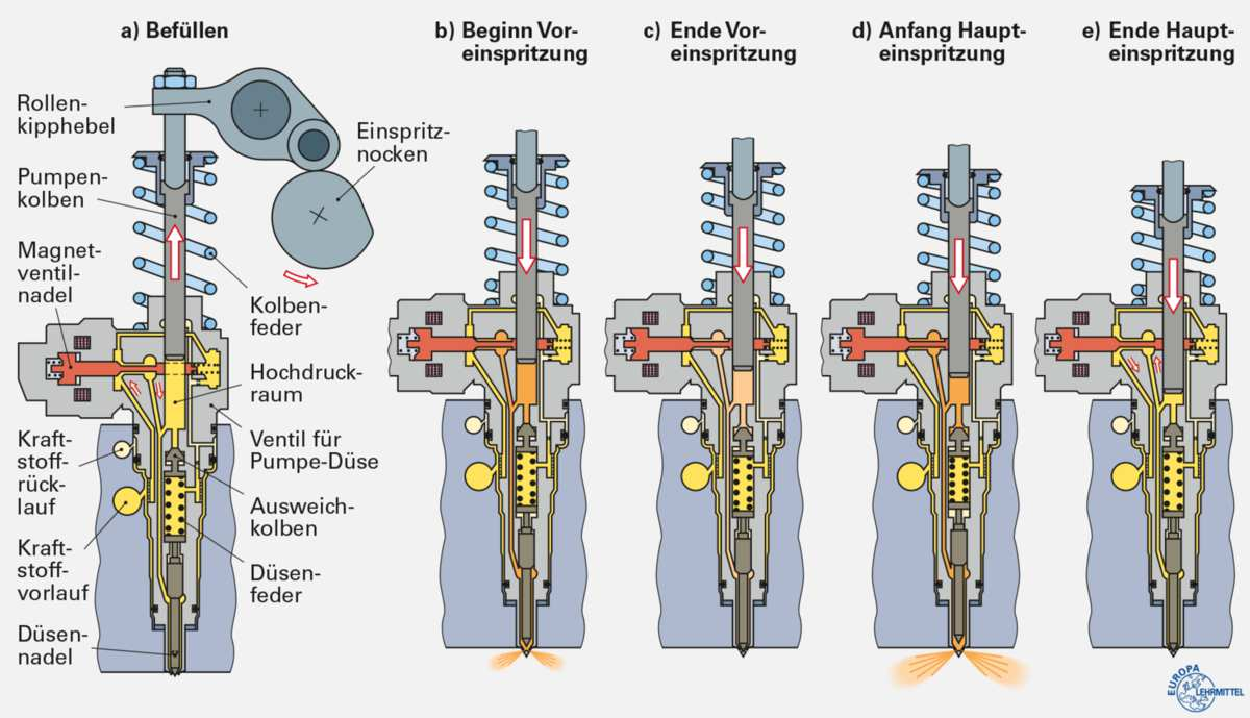
\includegraphics[width=0.7\textwidth]{images/Diesel/Diesel-11.pdf}
\caption{Pumpe-Düse System, Quelle: Europa-Verlag}
%\label{fig:}%% anpassen
\end{figure}

\begin{enumerate}
\item
  Drallkanal
\item
  Füllkanal
\item
  Auslasskanal
\item
  Einlassnockenwelle
\item
  Kraftstoffrücklauf
\item
  Auslassnockenwelle mit Einspritznocken
\item
  Kolbenfeder
\item
  Einspritznocke
\item
  Rollenkipphebel
\item
  Ausweichkolben
\item
  Pumpenkolben
\item
  Magnetventil PDE
\item
  Einstellschraube Spielausgleich PDE
\item
  Kraftstoffzulauf
\item
  Hochdruckraum
\end{enumerate}

\textbf{Einspritzvorgang}

\begin{enumerate}
\item
  Nockenhub wird über den Rollenkippebel auf den Pumpenkolben übertragen
\item
  \textbf{Magnetventil angesteuert} und verschließt Kraftstoffzulauf und
  -rücklauf
\item
  Druckaufbau im Hochdruckraum beginnt
\item
  Bei ca. 180 bar ist der Druck größer als die Federkraft.
  \textbf{Voreinspritzung beginn}
\item
  Ausweichkolben öffnet Ausgleichsraum, kurzer Druckabfall.
  \textbf{Voreinspritzung ende}
\item
  Bei ca. 300 bar überwindet der Kraftstoffdruck die Kraft der
  vorgespannten Feder. \textbf{Haupteinspritzung beginn}
\item
  \textbf{Magnetventil nicht angesteuert} und öffnet den
  Kraftstoffzulauf und -rücklauf.
\end{enumerate}

\textbf{steile Flanke des Einspritznockens} bewirkt einen schnellen
Druckanstieg.

\subsection{Pumpe-Düse System mit
Piezoventil}\label{pumpe-duese-system-mit-piezoventil}

\textbf{Piezoelektrische-Effekt} (direkt), übt man auf einen
Piezokristall Druck aus, so erzeugt dieser eine Spannung.

\emph{Verformung} durch Druck / Krafteinfluss

\emph{Anwendung:} Klopfsensor, Drucksensor (Click-Feuerzeug)

\textbf{Reziproker Piezoelektrischer-Effekt} (invers) legt man an einen
Piezokristall eine Spannung an, so verformt er sich. Die Längenänderung
ist proportional zur angelegten Spannung.

\emph{Verformung} durch Spannungseinfluss

\emph{Anwendung:} Injektor

Kfz: Steuerspannung 110-150 V, max. Ausdehnung 0,15 \%

Piezoventil ersetzt Magnetventil (Trägheit - Magnetventil bewegt sich
zeitversetzt, weil der Magnetfeldaufbau gehemmt wird, durch
Gegeninduktion)

\textbf{Piezoventil (Piezoaktor)} besteht aus Piezoaktormodul und
Übersetzermodul (kl. Hebelwerk)

Die Längenausdehnung eines Piezokristalls liegt bei maximal 0,15 \%
(sehr gering). Werden, bis zu 500 Piezokristalle in Reihe geschaltet ist
die Gesamtausdehnung des Piezoaktormodul etwa 0,04 mm. Zum Erreichen der
erforderlichen Ventilöffnung von 0,1 mm wird ein kleines Hebelwerk,
sogenannte Übersetzermodul zwischen Piezoaktormodul und hydraulischen
Ventil geschaltet.

\textbf{Piezoventil geschlossen}, die Verbindung zwischen Hochdruckraum
zur Vor- und Rücklaufleitung ist unterbrochen. Hochdruck kann sich
aufbauen und es wird eingespritzt.

\textbf{Piezoventil offen}, die Verbindung zwischen Hochdruckraum zur
Vor- und Rücklaufleitung ist wieder hergestellt. Hochdruck entweicht und
der Einspritzvorgang ist beendet.

\section{Einspritzventile}\label{einspritzventile}

\begin{itemize}
\item
  Ein- und Zweifeder-Düsenhalter
\item
  Loch- und Zapfendüsen
\end{itemize}

\textbf{Prüfen:} Öffnungsdruck, Strahlbild

\section{Glühsysteme}\label{gluehsysteme}

\textbf{Aufgabe von Starthilfsanlagen}

\begin{enumerate}
\item
  Anspringen des kalten Dieselmotors erleichtern
\item
  runden und stabilen Leerlauf zu sorgen
\item
  Schadstoffemissionen zu senken
\end{enumerate}

\textbf{Arten von Glühstiftkerzen}

\begin{enumerate}
\item
  \textbf{Selbstregelnde Glühstiftkerzen}

  \begin{itemize}
  \item
    \emph{Aufbau:} Heizwendel, Regelwendel, Keramikstift, Ringspalt
  \item
    \emph{Nennspannung:} 11,5 V
  \item
    \emph{Vorglühzeit:} 2 -- 7 s
  \item
    \emph{Glühtemperatur:} $850^\circ\text{C}$
  \item
    \emph{Leistungsaufnahme:} 100 W
  \item
    \emph{Regelung der Glühkerzenstromaufnahme:} Durch das PTC-Verhalten
    der Regelwendel wird die Stromaufnahme nach erreichen der
    Glühtemperatur begrenzt.
  \end{itemize}
\item
  \textbf{Elektronisch geregelte Glühstiftkerzen}

  \begin{itemize}
  \item
    \emph{Aufbau:} Heizwendel, Regelwendel, Keramikstift, Ringspalt
  \item
    \emph{Nennspannung:} 5 -- 8 V
  \item
    \emph{Vorglühzeit:} 1 -- 2 s
  \item
    \emph{Glühtemperatur:} $1000^\circ\text{C}$
  \item
    \emph{Regelung der Glühkerzenstromaufnahme:} Die Glühkerzen werden
    pulsweitenmoduliert kurzfristig mit Überspannung von bis zu 11 V
    betrieben.
  \end{itemize}
\item
  \textbf{Drucksensorglühstiftkerzen} (PSG, Pressure Sensor Glow Plug,
  Brennraumdruckgeber)

  \begin{itemize}
  \item
    Einspritzzeitpunkt und Druckverlauf ermitteln
  \end{itemize}
\end{enumerate}


	%%%%%%%%%%%%%%%%%%%%%%%%%%%%%%%%%%%%%%%%%%%%%%%%%%%%%%%%%%%%%%%%%%
    % Bibliographie
    \printbibliography[category=cited]
\end{document}
